\documentclass[11pt, a4paper]{report}

\usepackage[final]{pdfpages}

	\usepackage{tikz}
\usetikzlibrary{arrows,calc,positioning,shadows,shapes,trees}

\tikzset{
  basic/.style  = {draw, text width=2cm, drop shadow, font=\sffamily, rectangle},
  root/.style   = {basic, text width=5cm, rounded corners=2pt, thin, align=center,
                   fill=green!30},
  level 2/.style = {basic, rounded corners=6pt, thin,align=center, fill=green!60,
                   text width=8em},
  level 3/.style = {basic, thin, align=left, fill=pink!60, text width=6.5em}
}

\usepackage{verbatim}

\usepackage{hyperref}

\title{\textbf{Seeker\\\normalsize{Project Documentation}}}
\author{Jaroslaw Hirniak}
\date{Last updated on: \emph{\today}}
\setcounter{tocdepth}{1}
\begin{document}

\maketitle

\tableofcontents

%--- Ch1: Project
\chapter{Project}
 
\section{Motivation}
% TODO: make more general
% TODO: move document data to document format section
\paragraph{}
The World Wide Web is rich source of information and many excellent search engines exist that help to find interesting information in the matters of seconds. However, they only provide the link to the source of information and if user wants to compare data from many sources or gather it for analysis is left with daunting task of collecting all this information by hand.

\paragraph{}
This is repetitive and daunting task, something that humans do not like, but computers love. It would be much better to let computer prepare data for the analysis for human and let human do the creative work.

\paragraph{}
The goal of this project is to research method and develop application to generate aggregate documents composed of sections of interest extracted from many sources (e.g. PDF, DOC, HTML, etc.) with proper annotations (about sources and their version) and provide those documents for analysis by humans.

\section{Proof of concept}
\paragraph{}
The project idea originated as a solution to a problem faced by the researches in minority languages at the University of Edinburgh, who faced issue of gathering data from \href{http://www.coe.int/t/dg4/education/minlang/Report/default_en.asp}{European Charter for Regional or Minority Languages} website for comparative analysis and producing various reports based on that data.

\paragraph{}
Therefore, the proof of concept should solve the issue faced by the researches in minority languages, and provide them with a tool that enables easy aggregate document generation from source documents available on \href{http://www.coe.int/t/dg4/education/minlang/Report/default_en.asp}{European Charter for Regional or Minority Languages} website.

\section{Data sources}
\paragraph{}
The sources of data come from specified list of websites\footnote{However, it could be adapted for more general approach with web crawler searching for interesting kind of data, but that would involve scalability issues of storing and parsing such large data set and automatic recognition ofatRegional or Minority Languages} website, all of which are available in PDF format. There are 651 documents linked on the page, of which 309 documents are in English (some documents are produced also in French or country producing report official language), of which 300 documents are of actual interest (rest includes charter advertisements or more general texts). There are 25 countries producing reports, each adhering to general layout, but with subtle differences coming from the tool used or typesetting conventions, which should be taken into account during parsing PDF into JSON\footnote{The best parser would have simple regular expression and extract only relevant sections without specific formatting. This has been achieved for this project with context aware parser.}.

\section{Stakeholders}

\begin{itemize}
  \item Researchers - people who are using service often for their research;
  \item Consumers - people who need to access data occassionally and do not have need to register an account in the service;
  \item Administrators - people having rights to add sources, respond to tickets, etc.;
  \item Developer - person responsible for the project development and maintenance.
\end{itemize}

\section{Project Name}
The project name \emph{Seeker} comes from \href{http://www.scottishpoetrylibrary.org.uk/poetry/poems/seeker-reaper}{``Seeker, Reaper''} poem by \href{http://en.wikipedia.org/wiki/George_Campbell_Hay}{George Campbell Hay}. You can listen to the peom being recited on YouTube \href{https://www.youtube.com/watch?v=gjxPtRZFF24}{here}.

%---

%--- Ch2: Requirements

\chapter{Requirements}

\section{Minimal requirement}
The goal for 8 week summer project was set to
\begin{itemize}
  \item carry out research and recommend appropriate solution (architecture, full software stack, and persistence layer);
  \item Implement a proof of concept functionality to prove the possibility of developing efficient solution for the stated problem, this is, ability to query European Committee for Minority Languages and receive combined documents composed of elements specified in the query.
\end{itemize}

\section{Data format}
The main source of the data are going to be the European Charter for Regional or Minority Languages expert reports\footnote{\url{http://www.coe.int/t/dg4/education/minlang/Report/default_en.asp}}.

The goal of the project is to account for the future grow and to include also documents from Galeic Plans produced by various bodies in Scotland \footnote{http://www.gaidhlig.org.uk/bord/en/our-work/gaelic-language-plans.php}.

The data needs to be assumed to do not have any common format or fields.

\section{Use cases}
During the initial meeting on 26 May 2014 the below use cases had been identified.

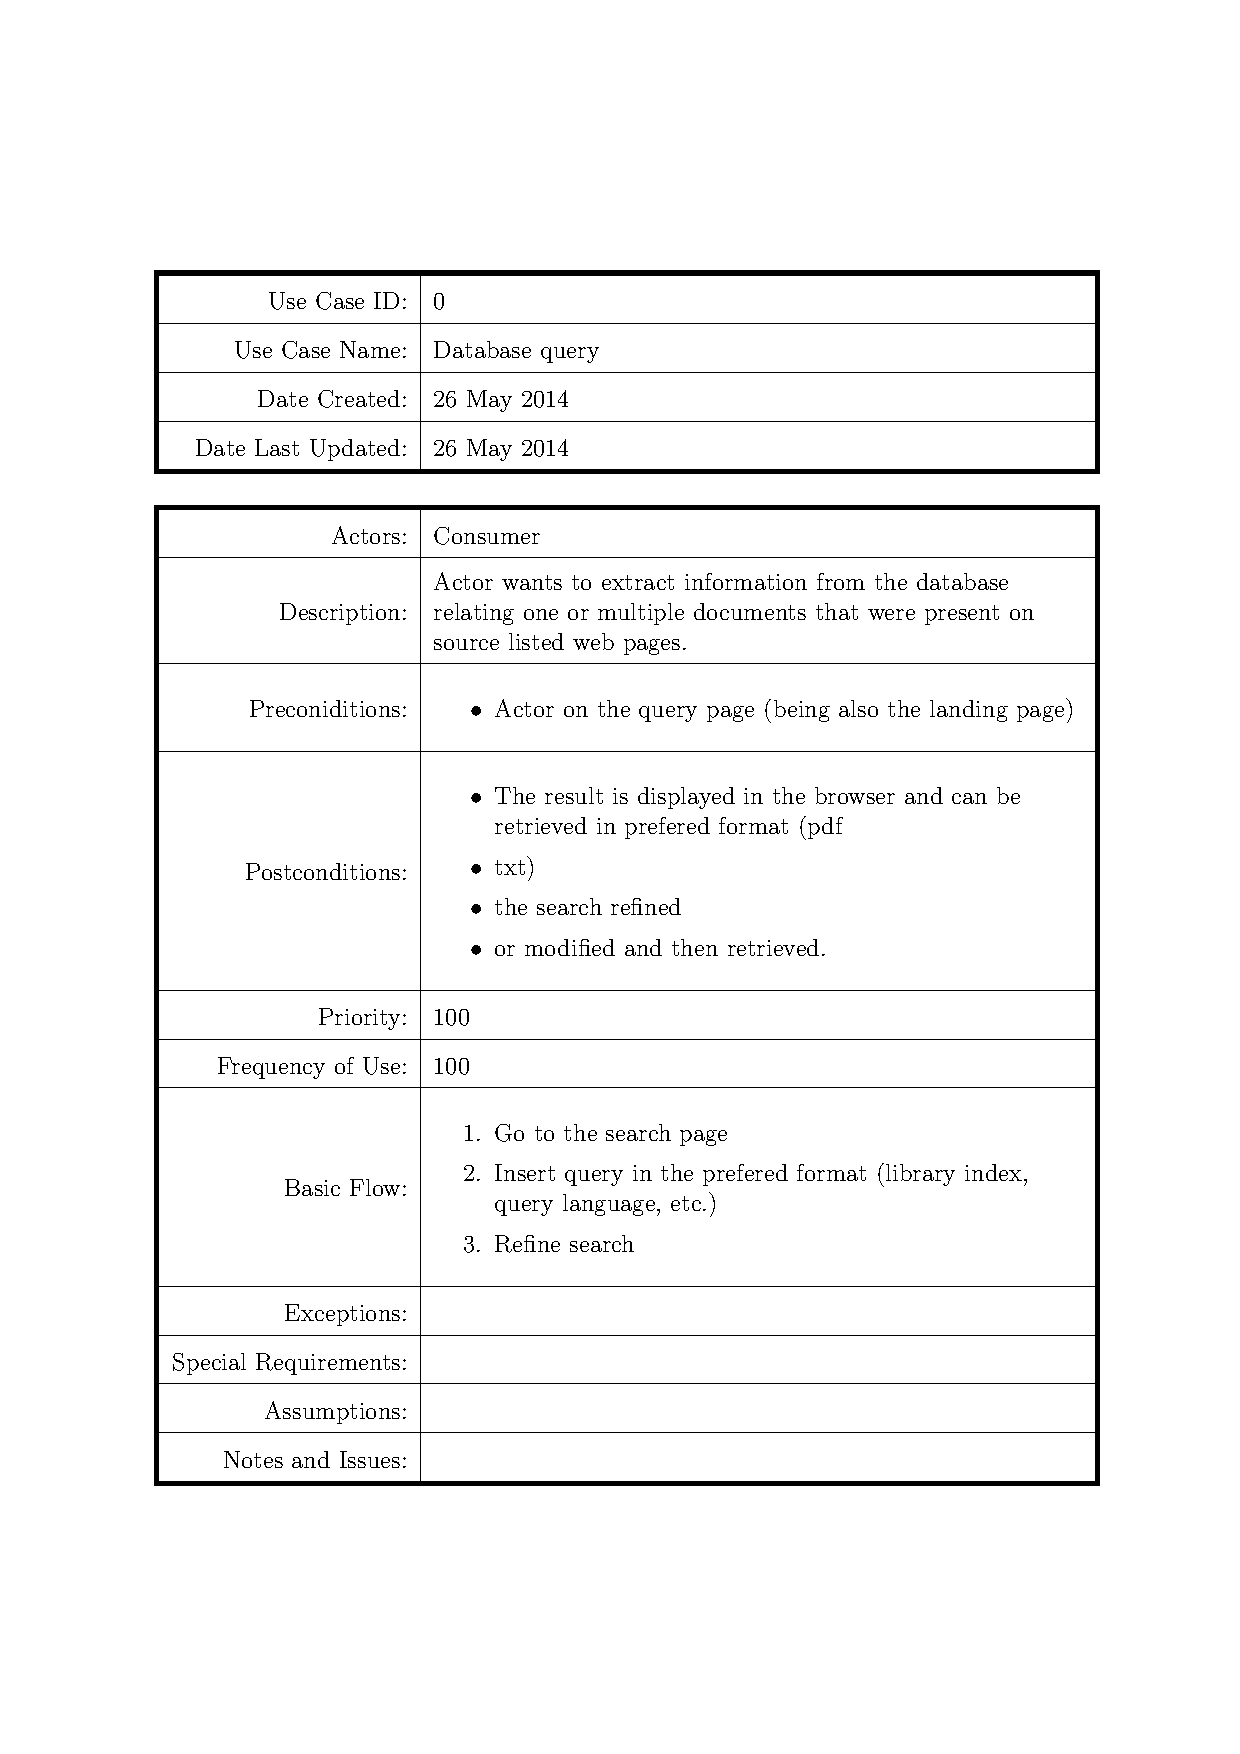
\includepdf[pages=1]{Requirements/UseCases/000_Query.pdf}
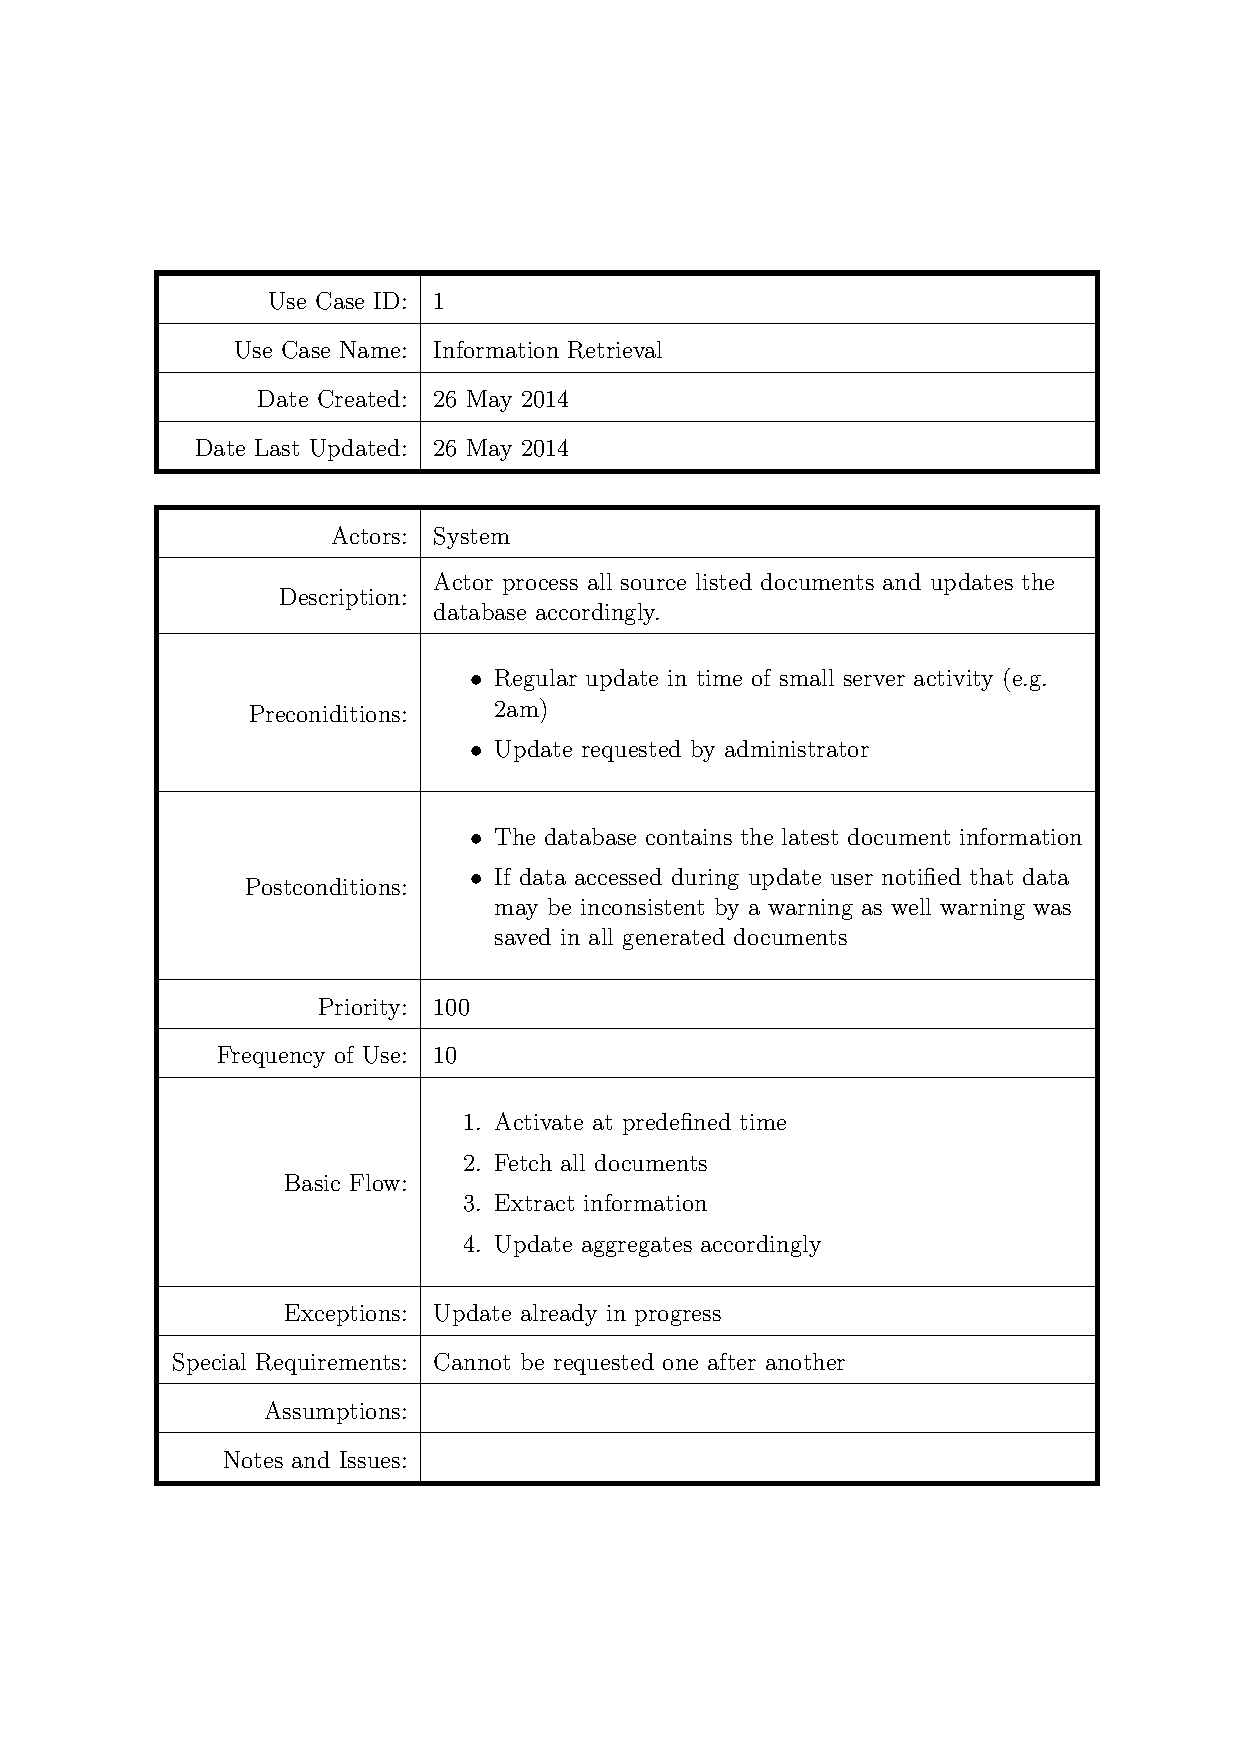
\includepdf[pages=1]{Requirements/UseCases/001_IR.pdf}
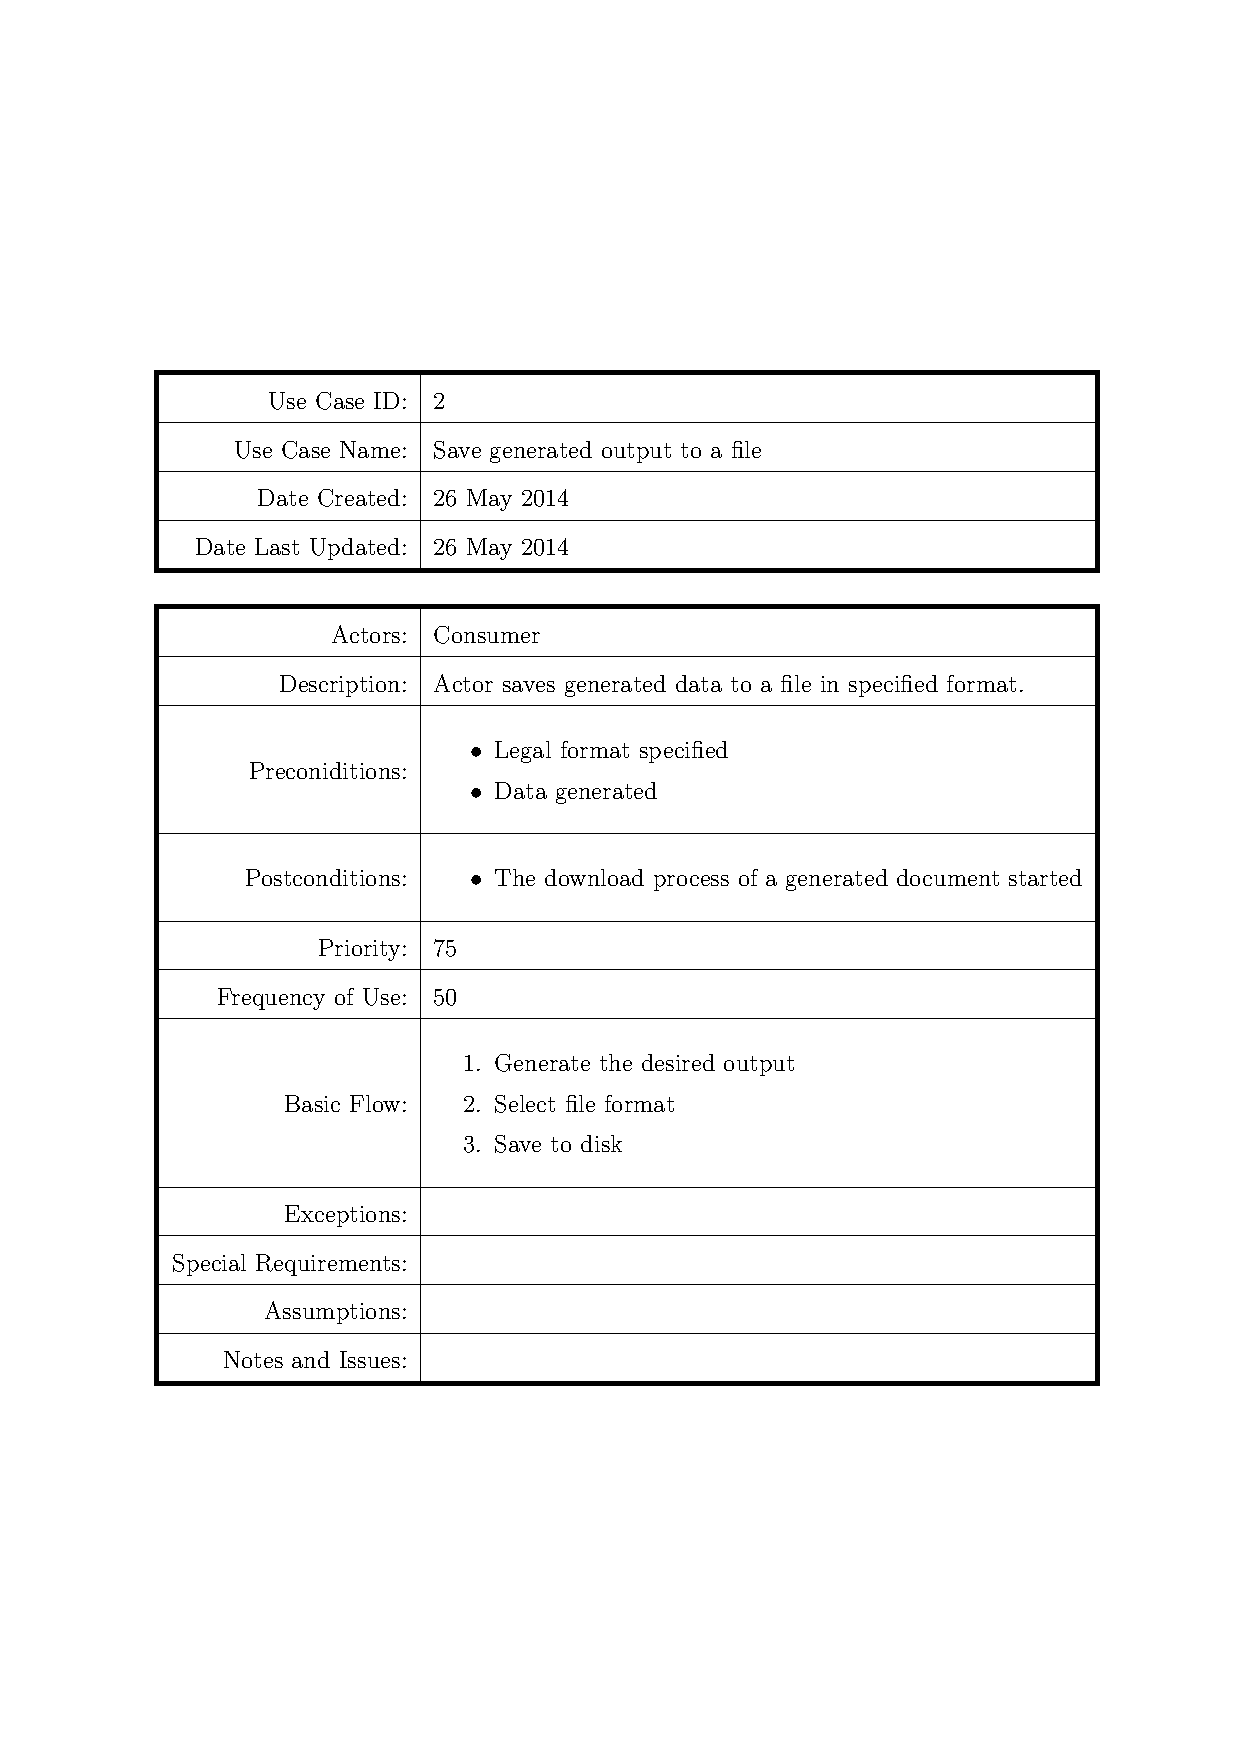
\includepdf[pages=1]{Requirements/UseCases/002_SaveOutput2File.pdf}
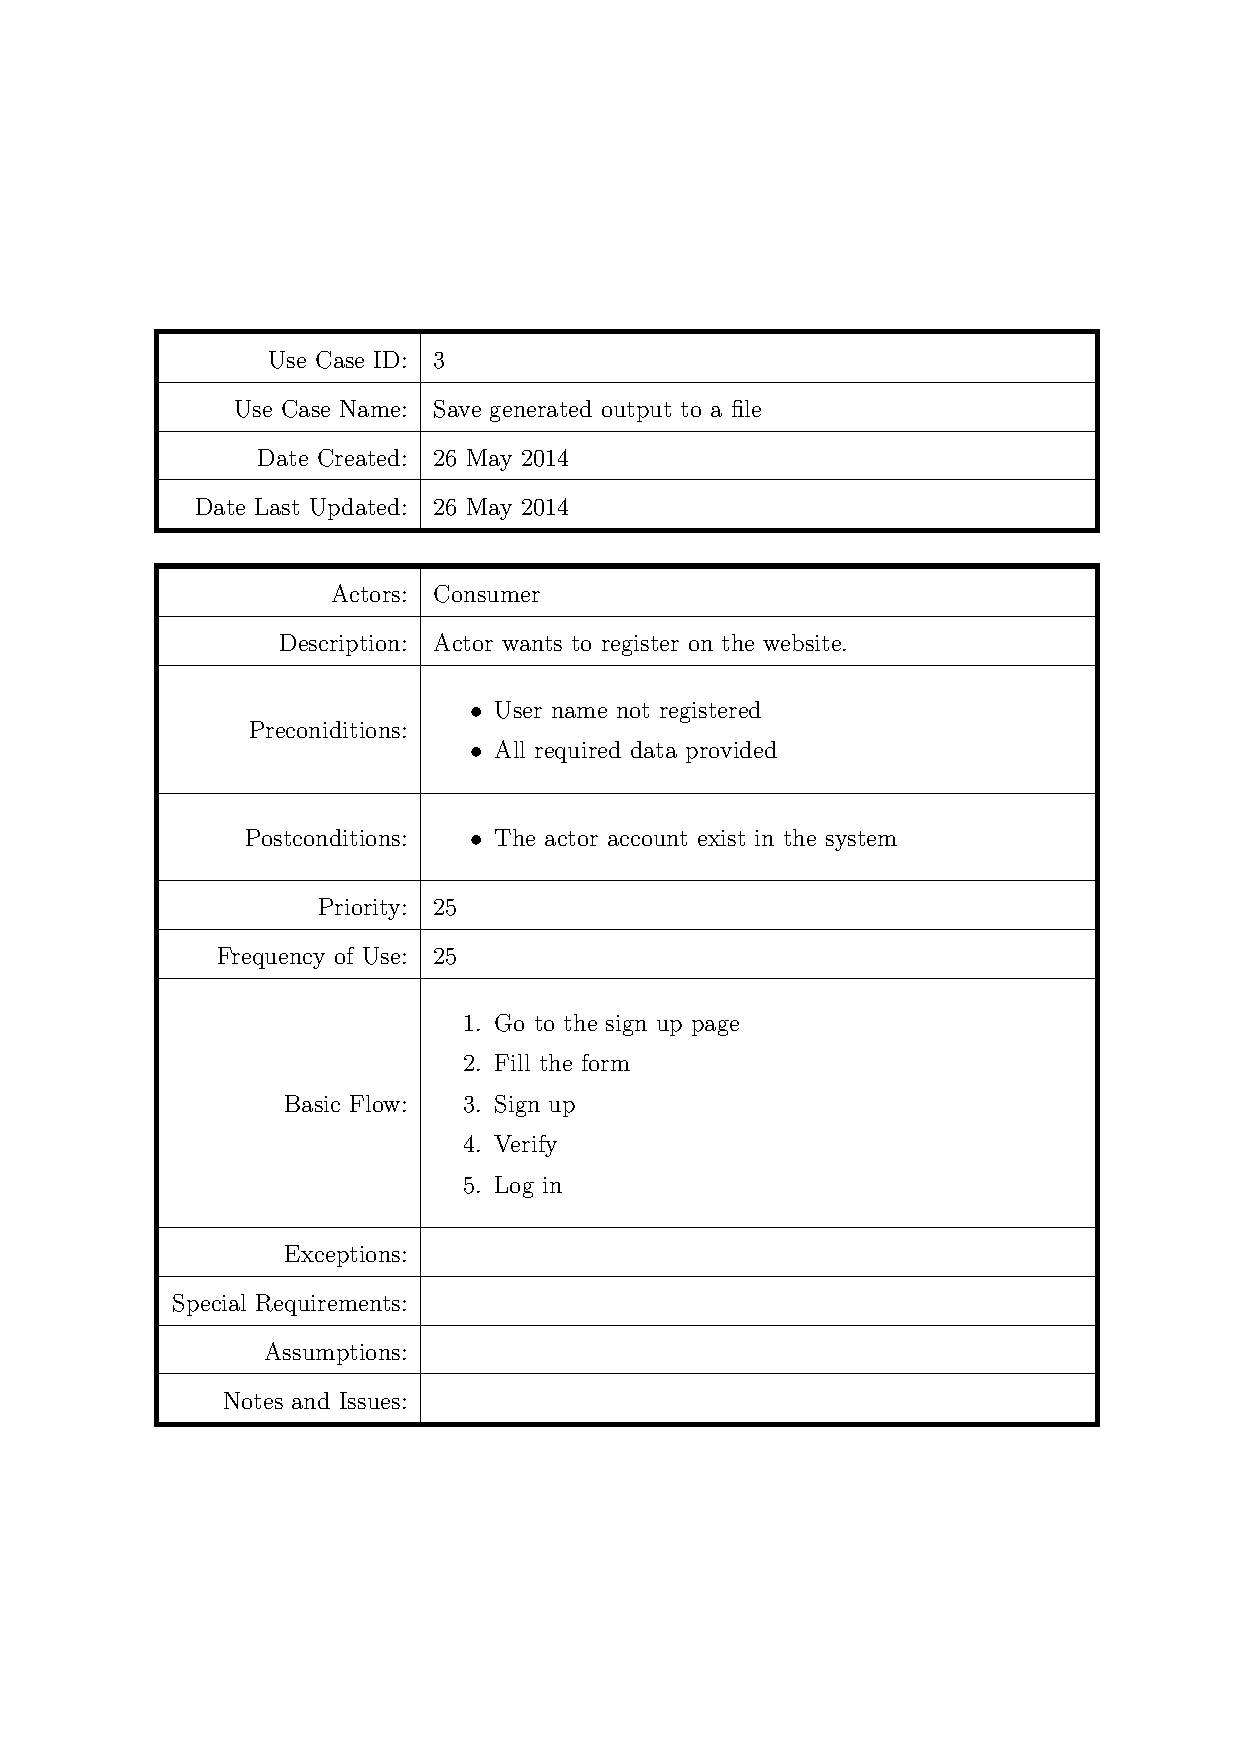
\includepdf[pages=1]{Requirements/UseCases/003_SignUp.pdf}
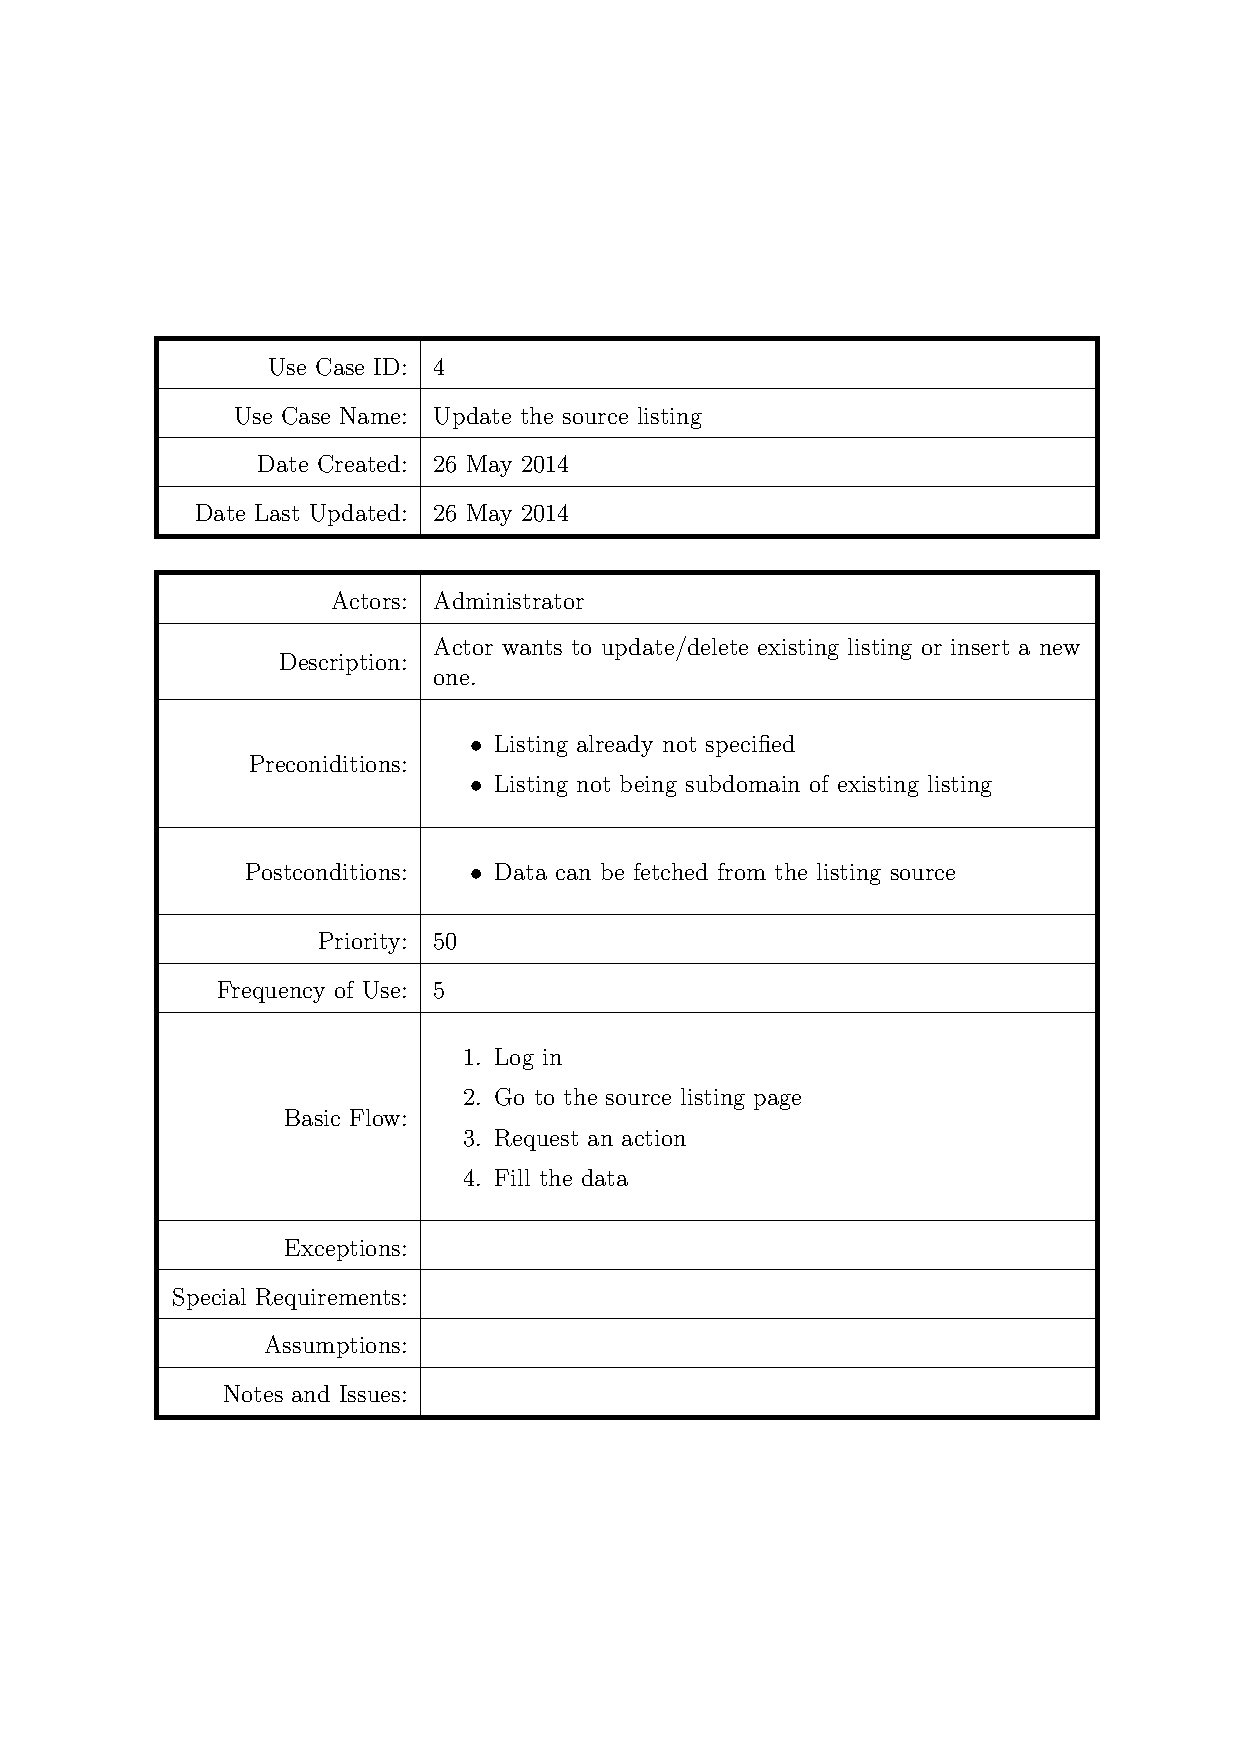
\includepdf[pages=1]{Requirements/UseCases/004_SourceListingUpdate.pdf}
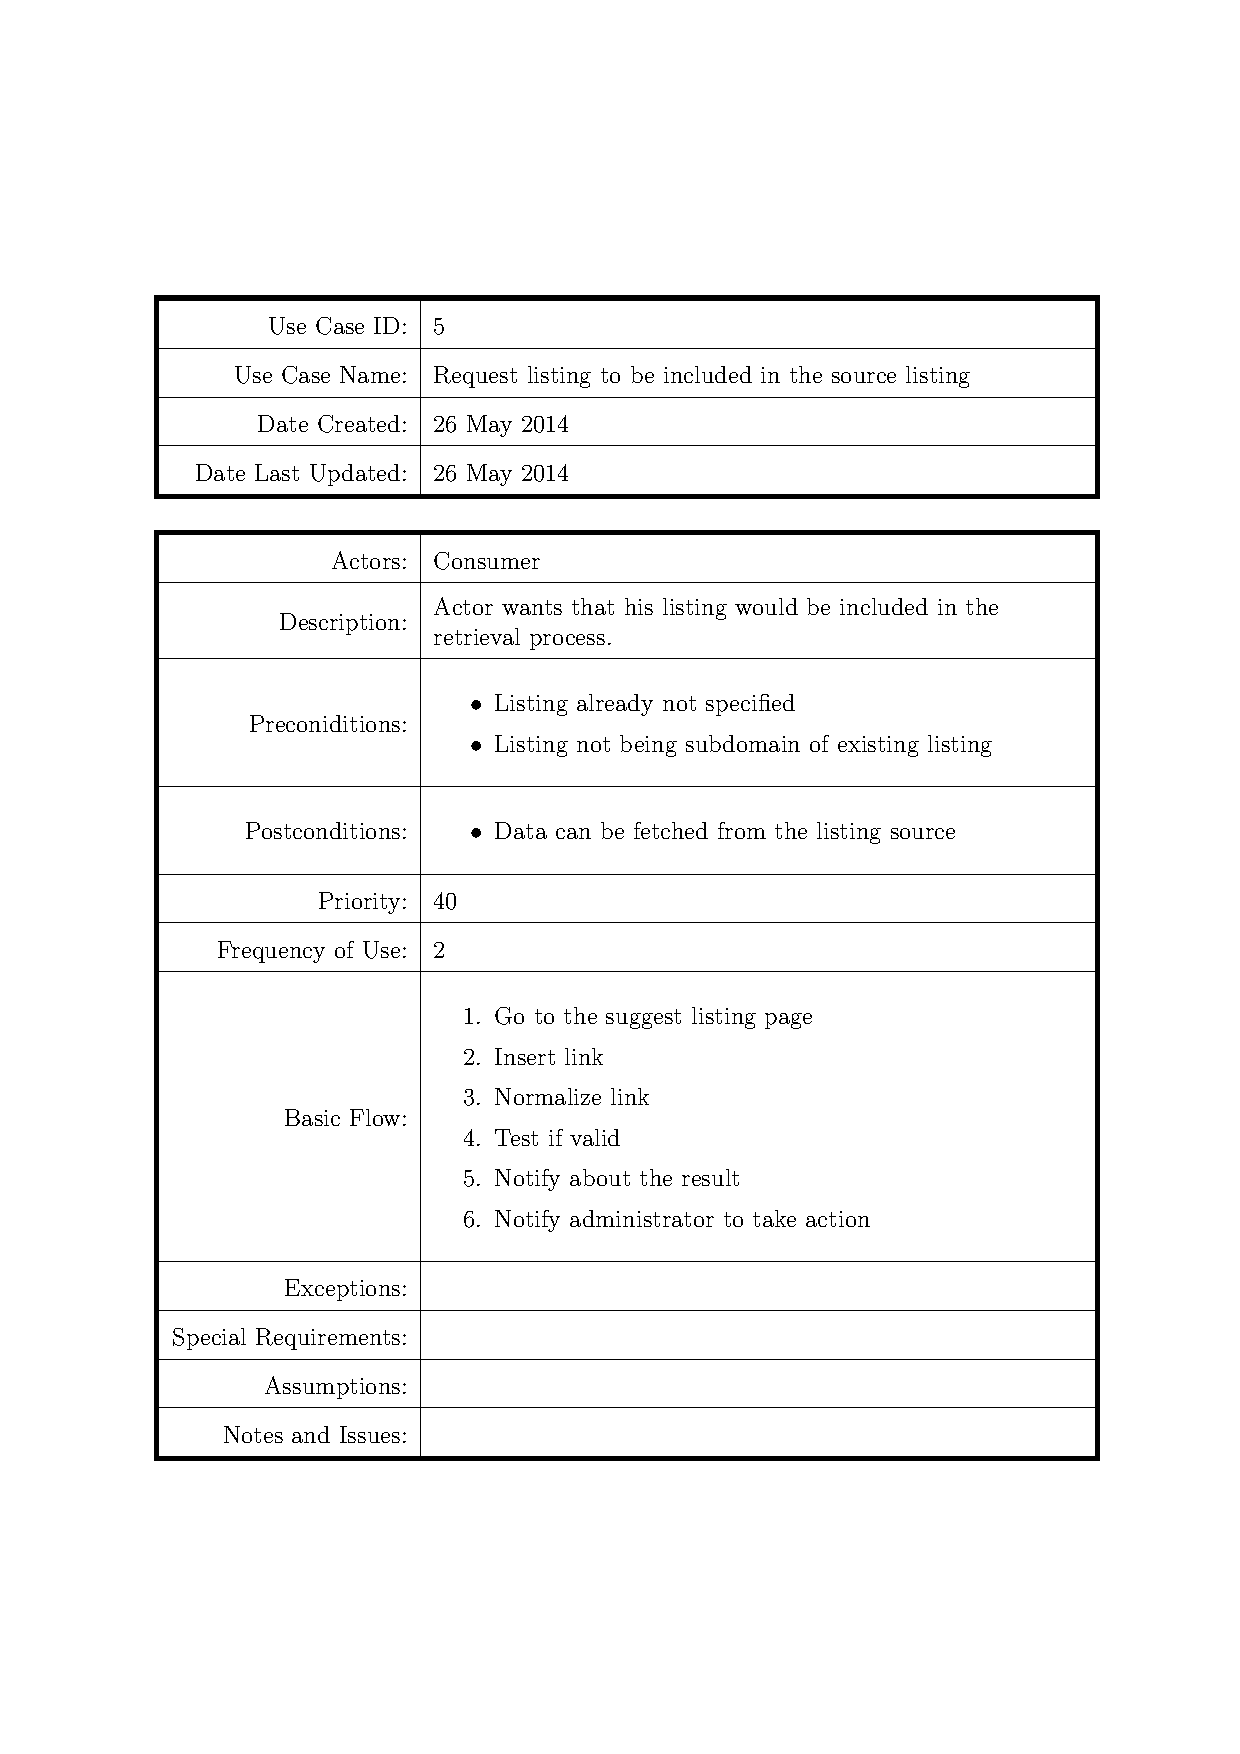
\includepdf[pages=1]{Requirements/UseCases/005_RequestListingToBeIncluded.pdf}
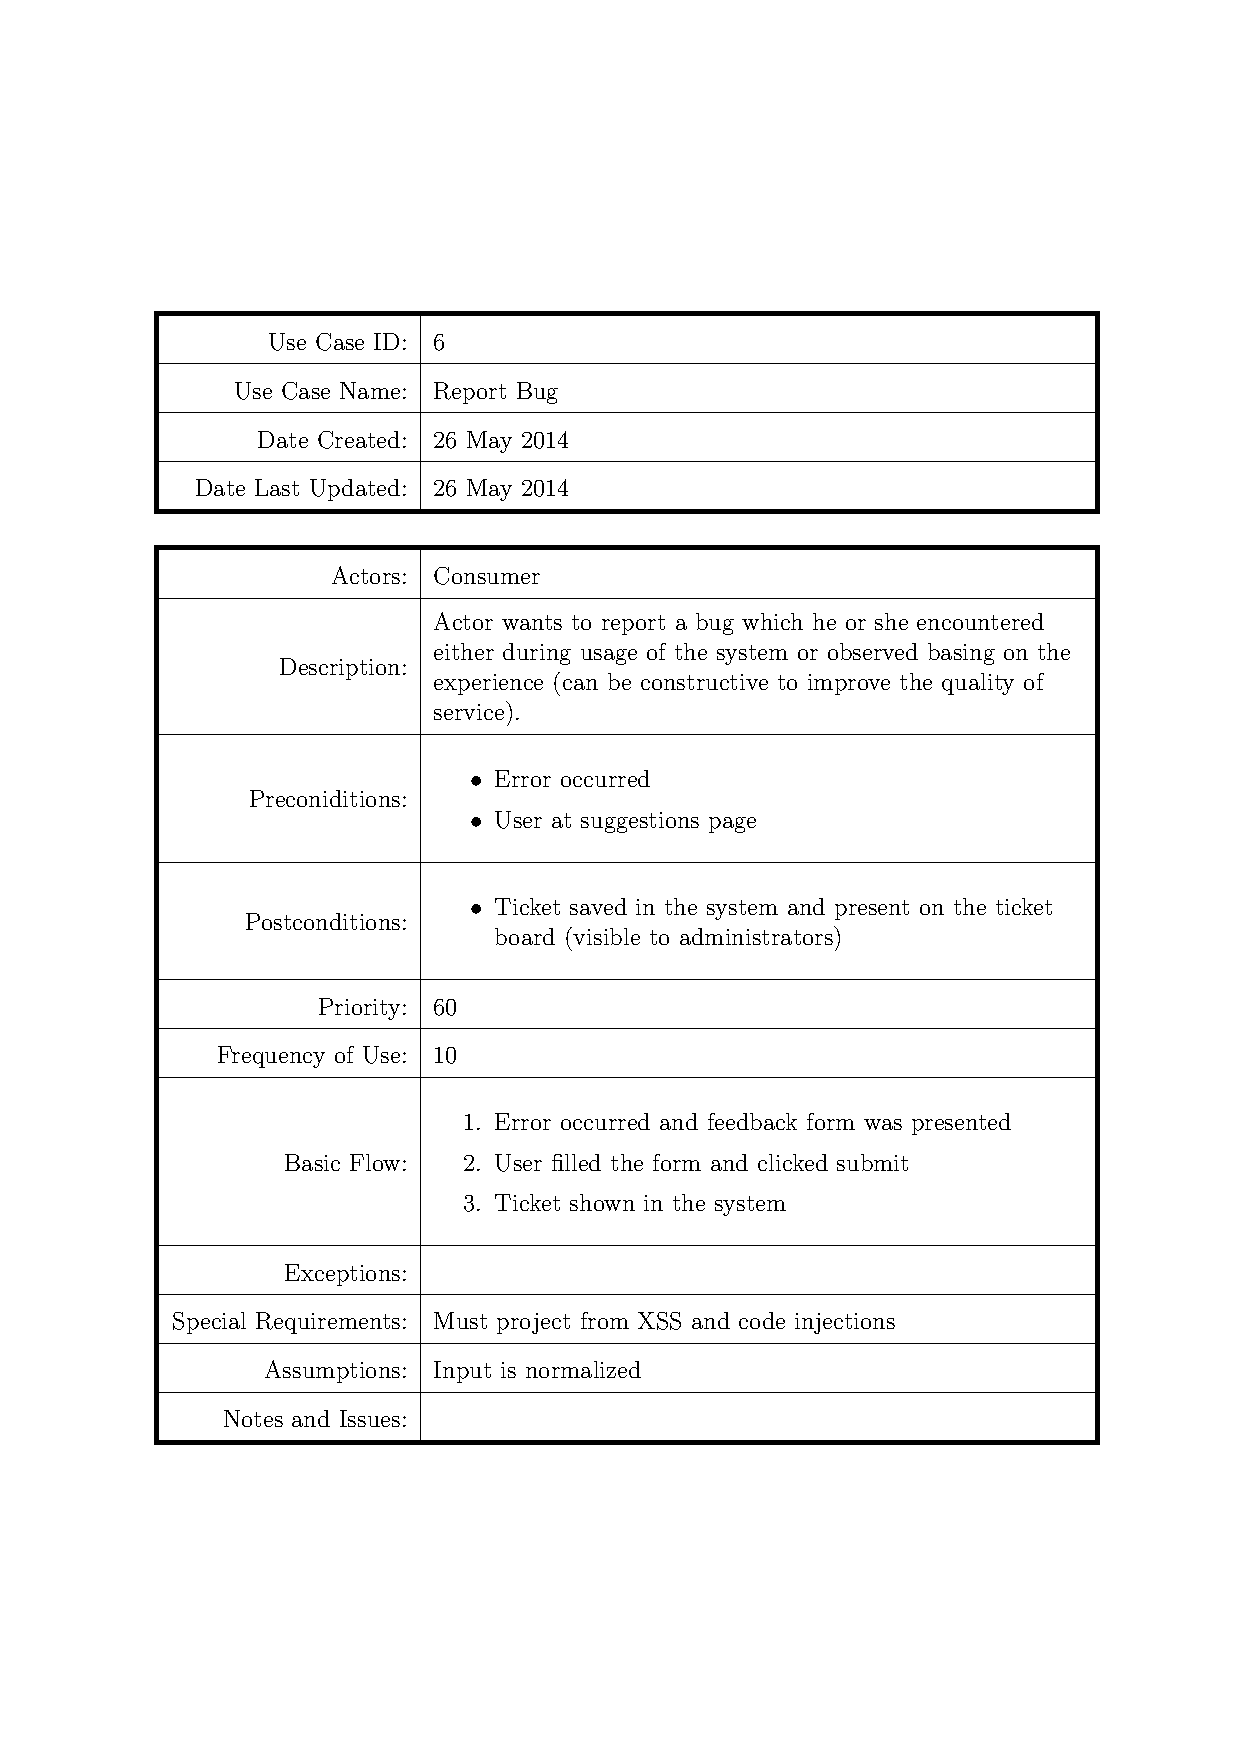
\includepdf[pages=1]{Requirements/UseCases/006_ReportBug.pdf}

%---

%--- Ch3: Requirement analysis
\chapter{Requirements analysis}

\section{Objectives}
\begin{itemize}
  \item Contiunable - the project development should be easy to continue
    \begin{itemize}
      \item Well-documented
      \item Popular and well-documented technologies should be used
      \item Well-organized code base
    \end{itemize}
  \item Schemaless - documents (sometimes even from the same source) will have different structure, so it is important to not restrict the database to store one kind (structure) of information
  \item Adaptability - it shoud be easy to adapt a project to a new kind of documents/task
  \item Modularity - the distinguishable project parts should be implemented in modular fashion to increase clarity and make the future development easier
  \item Open source - all technologies and tools used should be open source
\end{itemize}

\section{Data layer}
\subsection{Example query}
\begin{enumerate}
  \item Show all Committee of Experts recommendations under article 7b.
  \item Show all sections relating to Scottish Gaelic.
\end{enumerate}

\subsection{Options}
The following database technologies were taken into consideration:
\begin{itemize}
  \item Traditional RDMS such as PostreSQL and MySQL
  \item Key-value store such as Riak and Redis
  \item Document database such as MongoDB and CouchDB
  \item Graph database such as Neo4J and Infinite Graph
\end{itemize}

\paragraph{Traditional RDMS} has drawback of dedicated to the outlined schema and every new document (not to mention every new source of documents) has a chance to have different organization than the previous ones.

\paragraph{Key-value store} has not enough good query languages and 

\paragraph{Document database} has both flexible structure of aggregates (so we are not dedicated to one schema) and powerful query language (which can be implemented using incremental update)

\paragraph{Graph database} has ability to perform rich queries regarding relationships, but is not as powerful when it comes to queries relating the content, can answer queries like 1 and 2 in O(1) time, but update is expensive.

\subsection{Choice}
MongoDB has been chosen for storing documents because
\begin{itemize}
  \item it has big community of supporters and developers;
  \item it is well-documented;
  \item naturally blends with JavaScript when implementing query (JQuery notation) and data from the database (JSON);
  \item can store and operate on big documents of varying schema easily
  \item has rich query language with greater capabilities than the need outlined in the example queries subsection;
  \item when used with Node.js increases programmers productivity significantly (one language, centralized view)
\end{itemize}

When developing session and account management functionality it would be beneficial to implement the concept of polyglot persistence and for these two use key-value database, which creates separation of the concers as well as suits better the case.


\section{Application layer}
\subsection{Example usage}

\subsection{Options}
Three programming languages/frameworks were considered as potentially suitable for the project, namely:
\begin{itemize}
  \item Java and JSP
  \item Python and Django
  \item JavaScript and Node.js
\end{itemize}

\paragraph{Java and JSP} does not support well the programmer productivity as to perform even the simplies operations it is very expressive. When used the application needs to be developed and tested as a whole, so it does not support modularity and extendability well. The data layer technology of choice provides API for the language, but it is rather easier and more natural to operate on it in JavaScript than in Java.

\paragraph{Python and Django} had the same drawbacks, except it provides greater productivity.

\paragraph{JavaScript and Node.js} means that one language would be used for front-end and back-end, including data quering and manipulation, what highly increases the programmer productivity. Further, JavaScript as front-end language provides rich choice of libraries like jQuery, Angular, etc. that can be used to further increase productivity and presentation quality. When it comes to the back-end all operations are handled efficiently using event-loop. The aggregates are retrieved in JSON format and MongoDB can be naturally quiered using jQuery like notation. This all results in complete and efficient solutioon.

\subsection{Choice}

Node.js has been chosen for the front-end and back-end development because
\begin{itemize}
  \item it integrates well with MongoDB
  \item enables using one language for everything (front-end, back-end, database);
  \item is efficient 
\end{itemize}

%---

%--- Ch4: Architecture
\chapter{Architecture}

\section{Overview}

\subsection{Application}

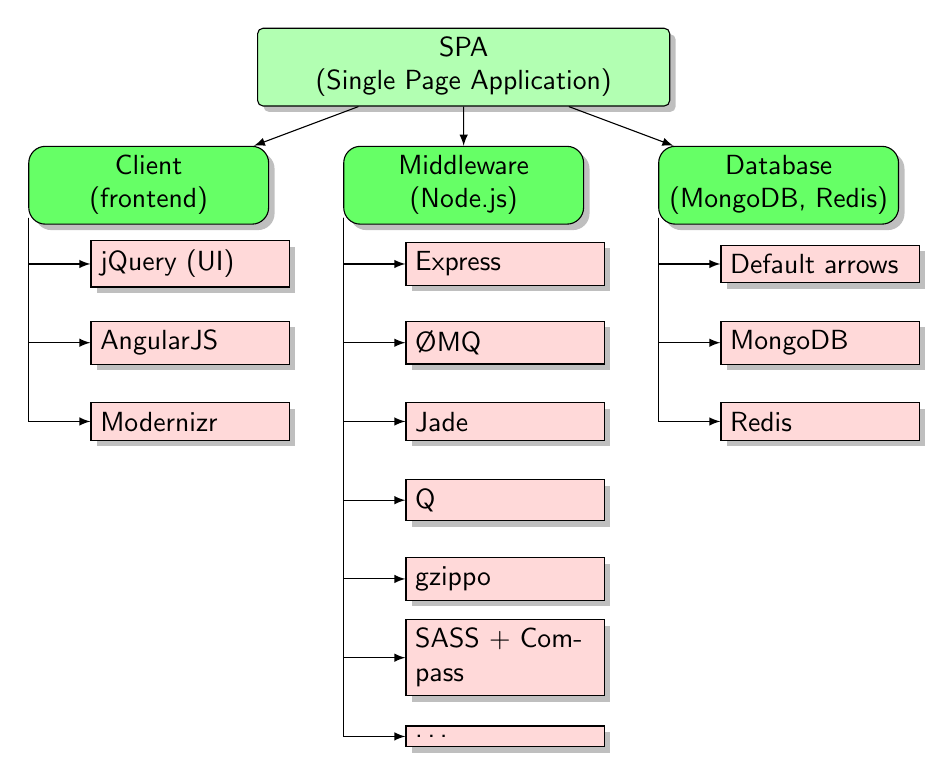
\begin{tikzpicture}[
  level 1/.style={sibling distance=40mm},
  edge from parent/.style={->,draw},
  >=latex]

% root of the the initial tree, level 1
\node[root] {SPA\\\mbox{(Single~Page~Application)}}
% The first level, as children of the initial tree
  child {node[level 2] (c1) {Client\\(frontend)}}
  child {node[level 2] (c2) {Middleware (Node.js)}}
  child {node[level 2] (c3) {Database \mbox{(MongoDB,~Redis)}}};

% The second level, relatively positioned nodes
\begin{scope}[every node/.style={level 3}]
\node [below of = c1, xshift=15pt] (c11) {jQuery (UI)};
\node [below of = c11] (c12) {AngularJS};
\node [below of = c12] (c13) {Modernizr};

\node [below of = c2, xshift=15pt] (c21) {Express};
\node [below of = c21] (c22) {{\O}MQ};
\node [below of = c22] (c23) {Jade};
\node [below of = c23] (c24) {Q};
\node [below of = c24] (c25) {gzippo};
\node [below of = c25] (c26) {SASS + Compass};
\node [below of = c26] (c27) {\dots};

\node [below of = c3, xshift=15pt] (c31) {Default arrows};
\node [below of = c31] (c32) {MongoDB};
\node [below of = c32] (c33) {Redis};
\end{scope}

% lines from each level 1 node to every one of its "children"
\foreach \value in {1,2,3}
  \draw[->] (c1.195) |- (c1\value.west);

\foreach \value in {1,...,7}
  \draw[->] (c2.195) |- (c2\value.west);

\foreach \value in {1,...,3}
  \draw[->] (c3.195) |- (c3\value.west);
\end{tikzpicture}

Description
\begin{itemize}
\item [\textbf{Client:}]
  \item jQuery (UI)
  \item AngularJS
  \item Modernizr

\item [\textbf{Middleware:}]  
  \item Express - main framework for message passing and service the content to the clients
  \item {\O}MQ - for message passing, mainly for efficient Router/Dealer protocol implementation
  \item Jade - for more productivity in templating
  \item gzippo - for serving gzipped content
  \item SASS + Compass - styling, plus features like building sprites out of files

\item [\textbf{Database:}]
  \item MongoDB - document data store for document management \emph{TODO}
  \item Redis - key-value data store for session and user data management
\end{itemize}

\subsection{Full layer}
% TODO: Add packages description and links to the project websites, and icons :)
\emph{Picture showing Yeoman, Grunt, Karma testing with Jasmin, etc.}
code: sudo npm install -g yo \# installs yeoman, grunt, bower, etc. globally
sudo npm install -g generator-angular-fullstack \# install angular generator (btw the most popular generator)
yo angular-fullstack seeker (projectname)\# create full stack locally with jade tempalates
[?] Would you like to use Sass (with Compass)? Yes                               │
[?] Would you like to include Twitter Bootstrap? Yes                             │
[?] Would you like to use the Sass version of Twitter Bootstrap? Yes             │
[?] Which modules would you like to include?                                     │
‣⬢ angular-resource.js                                                           │
 ⬢ angular-cookies.js                                                            │
 ⬢ angular-sanitize.js                                                           │
 ⬢ angular-route.js 
 mongo with mongosee
 passport 
 All yeses
\subsection{Code management and deployment process}

\section{Full stack}
\subsection{Client facing}
\subsection{Middleware}
\subsection{Persistence data store}


\section{System design}

\section{Query language}

\subsection{Elements}
\begin{itemize}
  \item \emph{source documents} (e.g. Committee of Experts reports)
  \item \emph{document specifiers} (e.g. cycle, country producing the document)
  \item \emph{selectors} (i.e., languages, sections, words)
  \item \emph{organizer} specifying how to structure the output document (e.g. arrange by section numbers, in each section by countries alphabetically)
  \item \emph{template} choose how to style the output document
\end{itemize}

\subsection{Dependencies as tree}
\begin{enumerate}
  \item \emph{Source documents} must be root.
  \item \emph{Document specifiers} can be children of each another, but can occur only once on any path from root to leaves, can appear multiple times.
  \item \emph{Selectors} (i.e. languages, sections, words) can be children of any node, and they are always terminal (leaves).
  \item \emph{Organizers}, \emph{templates}, and other similar options which can be added in the future must be children of root, and in case of \emph{organizers} they must be aware of all root's children except itself to display available options.
\end{enumerate}

\subsection{Query evaluation stages}
\begin{enumerate}
  \item Select relevant documents using:
  \begin{itemize}
    \item producer - group (e.g. committee)
    \item producer - origin, i.e. countries (e.g. UK)
    \item cycles - time (e.g. last)
  \end{itemize}
  \item filter the document content using selectors (i.e. sections, languages, filters- words, phrases, etc.)
  \item reorganize resulting JSON using organizers
  \item render using template
\end{enumerate}


%---
% Ch5: Implementation

\section{Implementation}
\subsection{Core}
% node.js + zmq + angularjs + mongodb ^ mongoose
\subsection{Rendering}
% compass + Sass
\subsection{Auxiliary modules}

%---
% Ch6: Deployment

\section{Deployment}
\subsection{Hosting Environment}
% vm on plaistow
% config
\subsection{Connecting to the server}
% ssh into user -> telnet into seeker/plaistow (machine)
\subsection{Managing Modules}
% localization due to restricted privileges
\subsection{Deployment Cycle}
% test -> sync -> restart
\subsection{Testing}
% test server
\subsection{Persistence}
% auto reboot with grunt.js

%---
% Ch7: Available data

\section{Data}

%---
% Ch8: Project perspectives

\section{Perspectives}

\end{document}